
\documentclass[journal,transmag]{IEEEtran}
\hyphenation{op-tical net-works semi-conduc-tor}

\usepackage{enumitem}

\usepackage{amsmath}


% *** GRAPHICS RELATED PACKAGES ***
%
\ifCLASSINFOpdf
   \usepackage[pdftex]{graphicx}
  % declare the path(s) where your graphic files are
  % \graphicspath{{../pdf/}{../jpeg/}}
  % and their extensions so you won't have to specify these with
  % every instance of \includegraphics
  % \DeclareGraphicsExtensions{.pdf,.jpeg,.png}
\else
  % or other class option (dvipsone, dvipdf, if not using dvips). graphicx
  % will default to the driver specified in the system graphics.cfg if no
  % driver is specified.
  % \usepackage[dvips]{graphicx}
  % declare the path(s) where your graphic files are
  % \graphicspath{{../eps/}}
  % and their extensions so you won't have to specify these with
  % every instance of \includegraphics
  % \DeclareGraphicsExtensions{.eps}
\fi
% graphicx was written by David Carlisle and Sebastian Rahtz. It is
% required if you want graphics, photos, etc. graphicx.sty is already
% installed on most LaTeX systems. The latest version and documentation
% can be obtained at: 
% http://www.ctan.org/pkg/graphicx
% Another good source of documentation is "Using Imported Graphics in
% LaTeX2e" by Keith Reckdahl which can be found at:
% http://www.ctan.org/pkg/epslatex
%
% latex, and pdflatex in dvi mode, support graphics in encapsulated
% postscript (.eps) format. pdflatex in pdf mode supports graphics
% in .pdf, .jpeg, .png and .mps (metapost) formats. Users should ensure
% that all non-photo figures use a vector format (.eps, .pdf, .mps) and
% not a bitmapped formats (.jpeg, .png). The IEEE frowns on bitmapped formats
% which can result in "jaggedy"/blurry rendering of lines and letters as
% well as large increases in file sizes.
%
% You can find documentation about the pdfTeX application at:
% http://www.tug.org/applications/pdftex





\begin{document}

\title{\textsc{Análisis y simulación del modelo Point Foot Walker para la marcha humana}}

\author{
\IEEEauthorblockN{Juan David Castro Bocarejo , Juan Camilo Hernandez Torres, William Andrés Gómez Roa}
\IEEEauthorblockA{Pontificia Universidad Javeriana, Bogotá, Colombia}
\IEEEauthorblockA{Proyecto Análisis de Marcha - Sistemas Dinámicos}


}
% The paper headers
\markboth{Point Foot Walker. Abril 21~2023}%
{Shell \MakeLowercase{\textit{et al.}}: Bare Demo of IEEEtran.cls for IEEE Transactions on Magnetics Journals}
\IEEEtitleabstractindextext{%

	\begin{abstract}
	In this project, the point foot walker model was simulated using MATLAB. The aim was to analyze the walking dynamics of this model in terms of the angular positions, velocities, and accelerations of the legs during the gait cycle. Limitations on leg angles were included and the heelstrike event was considered for the transition between gait cycles. It was found that the dynamics of the point foot walker are highly unstable, as expected from a real model. This study provides a basis for understanding the dynamics of the point foot walker and can be used to better understand the biomechanics of human gait. 
	\end{abstract}
	\begin{IEEEkeywords}
	Point foot walker, gait cycle, heelstrike, walking dynamics, biomechanics of gait.
	 	\end{IEEEkeywords}}


\maketitle
\IEEEdisplaynontitleabstractindextext
\IEEEpeerreviewmaketitle


\section{Resumen}
En este proyecto se simuló el modelo de caminador de pie puntal ‘point foot walker’ utilizando MATLAB. El objetivo fue analizar la dinámica de caminar de este modelo en términos de las posiciones, velocidades y aceleraciones angulares de las piernas durante el ciclo de la marcha. Se incluyeron limitaciones en los ángulos de las piernas y se consideró el evento de impacto del talón ‘heelstrike’ para la transición entre los ciclos de la marcha. Se encontró que la dinámica del caminador de pie puntal es altamente inestable como se espera de un modelo real. Este estudio proporciona una base para la comprensión de la dinámica del caminador de pie puntal y puede ser utilizado para entender mejor la biomecánica de la marcha humana.
\begin{IEEEkeywords}
	Caminador de pie puntual, ciclo de la marcha, golpe de talón, dinámica de la marcha, biomecánica de la marcha.
	 	\end{IEEEkeywords}

\section{Introduction}
La marcha humana es un fenómeno altamente complejo y ha sido objeto de estudio por décadas en campos como la biomecánica y la robótica \textbf{[1]}. Un modelo ampliamente utilizado en la investigación de la marcha humana es el Point Foot Walker, el cual consiste en dos piernas conectadas a una estructura rígida con un pie puntal en el extremo. Cada pierna se compone de dos segmentos, la pierna de apoyo o Stance leg y la pierna en movimiento o Spring leg, las cuales están conectadas en la cadera. La transición entre los ciclos de la marcha en este modelo ocurre cuando la pierna en movimiento se vuelve la pierna de apoyo y viceversa, y esto ocurre en un punto específico en la relación entre los ángulos theta y phi del modelo. Durante el evento de impacto del talón o heelstrike, se generan cambios significativos en las posiciones, velocidades y aceleraciones angulares de las piernas, lo que tiene implicaciones importantes en la biomecánica de la marcha humana \textbf{[2]}. 
	
	A continuación se da una descripción de los tipos de modelos de marcha humana:
	 \begin{itemize}
    \item \textit{Modelo péndulo invertido}: Es un modelo simplificado de marcha bipedal en el que se considera que las piernas son péndulos invertidos y el cuerpo es un péndulo simple. Este modelo es ampliamente utilizado en la investigación en locomoción bipedal debido a su simplicidad y su capacidad para capturar las dinámicas esenciales del movimiento humano \textbf{[1]}.
    \item \textit{Modelo tipo “compás” (Compass-like biped model)}: Es un modelo mecánico de la marcha bipedal en el que las piernas se mueven como un compás. Este modelo es útil para el análisis de los mecanismos de control de la locomoción bipedal y se ha utilizado en la investigación en la evolución de la locomoción humana y en el diseño de robots bipedales \textbf{[1]}.
    \item \textit{Ballistic walking} :Es un modelo de la marcha que considera que la locomoción humana se puede ver como una serie de saltos, cada uno de los cuales está controlado por un impulso inicial en la dirección adecuada. En este modelo, el cuerpo humano se divide en segmentos rígidos que se mueven como proyectiles. Esta técnica se basa en la conservación de la energía \textbf{[1]}.
    \item \textit{Active Dynamic walking}: Es una representación detallada del proceso de caminar humano que se basa en la dinámica de los músculos y la mecánica de los huesos y articulaciones. El modelo simula el comportamiento de los músculos y su capacidad para generar fuerza, lo que permite una mejor comprensión de los mecanismos subyacentes a la marcha. Además, este modelo puede ser utilizado para analizar cómo los cambios en los parámetros biomecánicos y neurológicos afectan la marcha, lo que es útil para la rehabilitación y el diseño de dispositivos de asistencia para la locomoción \textbf{[1]}.


    \textbf{¿Cuál es la limitación de la ley de Newton para el modelado de este tipo de sistemas?}
    La ley de Newton tiene limitaciones en el modelado de modelos reales complejos como la locomoción bipedal, ya que no tiene en cuenta la dinámica interna del sistema, como la energía potencial y cinética y la fricción en las articulaciones. 

    \textbf{Describir brevemente el método de Euler -Lagrange; ¿Cuál es la consideración básica en este método?} Básicamente el método de Euler-Lagrange consiste en encontrar una función Lagrangiana que describa la energía cinética y potencial del sistema y luego aplicar la ecuación de Euler-Lagrange para encontrar las ecuaciones dinámicas del sistema. 

    \textbf{Point foot Walker}
    Es un modelo mecánico simple de un caminador que se utiliza para estudiar la dinámica de la marcha humana. Este modelo consta de dos piernas rigidas sin articulación de rodilla, una de las cuales actúa como una pierna de apoyo mientras que la otra se mueve libremente. Las piernas se unen en la cadera cuya masa M representa la masa del cuerpo superior y es mucho mayor que la masa puntual de los pies, es por esto que en las ecuaciones se desprecian las masas \textbf{[2]}.El modelo está diseñado para imitar la marcha humana, y se utiliza comúnmente en la investigación de la biomecánica de la marcha.

    \textbf{Stance leg}
    Se refiere a la pierna que está en contacto con el suelo durante la marcha. Esta pierna soporta todo el peso del cuerpo y proporciona estabilidad durante la fase de apoyo de la marcha. La pierna de apoyo cambia continuamente durante la marcha, alternando entre la pierna izquierda y la pierna derecha \textbf{[2]}.

    \textbf{Spring leg}
    Se refiere a la pierna que no está en contacto con el suelo durante la marcha. Esta pierna se mueve libremente y se utiliza para impulsar el cuerpo hacia adelante durante la fase de oscilación de la marcha. La pierna de oscilación actúa como un resorte, almacenando energía durante la fase de apoyo y liberándola durante la fase de oscilación \textbf{[2]}.

     \textbf{Theta y Phi}
     Theta se refiere al ángulo entre la pierna de apoyo y la línea normal al suelo durante la fase de apoyo de la marcha. Phi se refiere al ángulo entre ambas piernas durante la fase de oscilación de la marcha. Estos ángulos son importantes para determinar la estabilidad y la eficiencia de la marcha \textbf{[2]}.

    \textbf{¿Para qué relación de ángulos ocurre la transición en la marcha?}
    La transición entre la fase de apoyo y la fase de balanceo de la marcha ocurre cuando los ángulos Theta y Phi cumplen la siguiente condición:
    		
	$\phi + 2\theta = 0 $

	Cuya condición entre estos ángulos esta dada para garantizar que la pierna de apoyo esté colocada correctamente en el suelo y proporcionar una base estable para el siguiente ciclo de la marcha.

    \textbf{Explicar los cambios que sufren las cuatro variables (las dos posiciones angulares y las dos
velocidades) cuando sucede el contacto del talón con el piso (heelstrike):}
 Cuando un pie golpea el suelo en el heelstrike, este tiene una colisión plástica (sin deslizamiento ni rebote) y su velocidad se vuelve cero. Ese pie permanece en el suelo, actuando como una bisagra, hasta que el pie que se balancea alcanza el golpe de talón. Al caminar, solo un pie está en contacto con el suelo en cualquier momento \textbf{[2]}.

Durante el contacto del talón con el piso o heelstrike, las cuatro variables (dos posiciones angulares y dos velocidades) experimentan cambios en su magnitud. La matriz de transición \textbf{A} describe estos cambios: 

\begin{equation*}
\begin{pmatrix}
\dot{\theta} \\
\ddot{\theta} \\
\dot{\phi} \\
\ddot{\phi} \\
\end{pmatrix}_{+} = 
\begin{pmatrix}
-1 & 0 & 0 & 0 \\
0 & \cos(2\theta) & 0 & 0 \\
-2 & 0 & 0 & 0 \\
0 & \cos(2\theta)(1-\cos(2\theta)) & 0 & 0 \\
\end{pmatrix}
\begin{pmatrix}
\theta \\
\dot{\theta} \\
\phi \\
\dot{\phi} \\
\end{pmatrix}_{-}
\end{equation*}


Específicamente, cuando se produce el heelstrike, la posición angular phi cambia a cero y la velocidad angular phi' cambia a su valor negativo. Por otro lado, la posición angular theta se mantiene constante, mientras que su velocidad angular theta' se vuelve negativa.

Estos cambios ocurren por la necesidad de ajustar las posiciones y velocidades angulares de las piernas durante el contacto del talón con el piso para mantener el equilibrio y permitir la transición a la fase de balanceo de la marcha.


\end{itemize}



%%%%%%%%%%%%%%%%%%%%%%%%%%INTRODUCCION


\section{Resultados y Análisis} 
Se simuló el modelo de caminador de pie puntal utilizando MATLAB y se analizó su dinámica en términos de las posiciones, velocidades y aceleraciones angulares de las piernas durante el ciclo de la marcha y se mostraron sus graficas con respecto al tiempo.  

Para esto, hicimos uso de las ecuaciones y teoría propuesta por \textbf{[1]}\textbf{[2]} para desarrollar nuestra simulación y replicar los resultados que se presentaron en dichos artículos:

\begin{equation}
\theta'' = \frac{g}{l} \sin(\theta - \lambda)
\end{equation}

\begin{equation}
\phi'' = \theta'' + \theta'^2 \sin(\phi) - \frac{g}{l} \cos(\theta - \lambda) \sin(\phi)
\end{equation}

Inicialmente, se realizó una simulación basada en el modelo planteado en el primer paper \textbf{[1]}, el cual no tomaba en cuenta la pendiente de inclinación del suelo $\lambda$. Este presentó curvas aproximadas a las presentadas en la sección de resultados como se observa en la figura \textbf{[1]}. 
Así mismo, esta simulación no toma en cuenta los estados de transición presentados en los métodos del paper, pues se realizó este proceso en la siguiente simulación.

\begin{figure}[!h]
		\center
		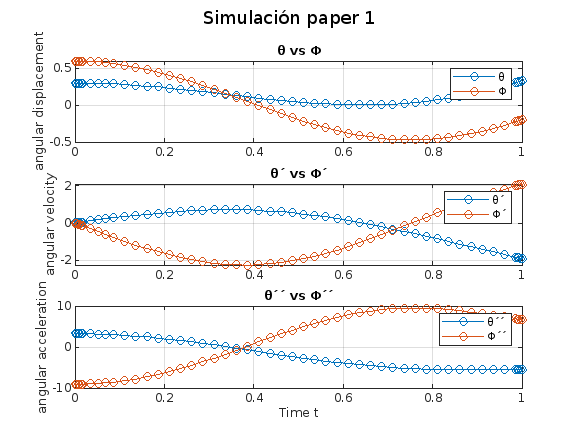
\includegraphics[width=9cm]{imgs/s1.png}
		\caption{Simulacion 1}
		\label{1}
\end{figure}


Ahora bien, se planteó un modelo más complejo con las especificaciones dadas en el segundo paper o paper original donde se describe el modelo \textbf{[2]}, así mismo se crearon funciones que simulaban el evento del heelstrike. Sin embargo, los modelos presentan saltos en la gráfica, los cuales de hecho tienen sentido con la matriz de transición mostrada en los papers, por lo que determinamos que probablemente sería necesario algún factor de corrección que no muestran en los artículos. Estos resultados se observan en la Figura \textbf{[2]}. 

\begin{figure}[!h]
		\center
		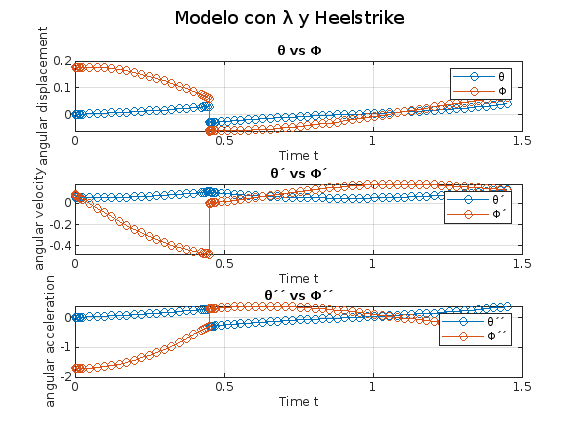
\includegraphics[width=9cm]{imgs/s2.png}
		\caption{Simulacion 2}
		\label{2}
\end{figure}

Acá se observa los cambios de magnitud en las variables al ocurrir el Heelstrike, asi como un cilco completo de la marcha a continuación de este. 

Si bien en los resultados de los artículos no se presentaron estos saltos causados por la función 'Heelstrike' esto se debe a que se limitaron a mostrar 1 único ciclo de la marcha y no mostraron los resultados de varios ciclos consecutivos. Nosotros hicimos la simulación del Hellstrike y concatenamos los resultados al ciclo anterior para poder observarlos en una sola gráfica.

Según \textbf{[2]}, se espera observar que la grafica de posición de phi y theta se cruzan en el punto 0 y ademas son simétricas con respecto a dicho punto. Cosa que se obtuvo en ambas simulaciones pero es más claro en la segunda simulación. 


  
%%%%%%%%%%%%%%%%%%%%%%%%%%%%%%%%%%%%%%%%%%%%%%%%%%%%RESULTADOS


\section{Conclusion}
	
	\begin{enumerate}[label=(\roman*)]

	 \item  Este proyecto contribuye a la comprensión de la biomecánica de la marcha y el análsis dinámico de sus variables, así como realizar la simulación del sistema biomecánico con la ayuda de Matlab. 

    \item  El modelo de caminador de pie puntal es un modelo simple pero útil para analizar la dinámica de la marcha humana. Aunque es altamente inestable, proporciona una base para la comprensión de la biomecánica de la marcha y puede ser utilizado para investigar diversos aspectos de la locomoción humana.
   

     \item  Los cambios que ocurren en las posiciones y velocidades angulares durante el contacto del talón con el piso (heelstrike) son consistentes con los patrones observados en la marcha humana. Estos resultados indican que el modelo de caminador de pie puntal puede ser utilizado para simular y analizar la dinámica de la marcha humana.

      \item  


	\end{enumerate}

\appendices


\ifCLASSOPTIONcaptionsoff
  \newpage
\fi


\begin{thebibliography}{1}


 \bibitem{IEEEexample1}
  Molina Arias, Ludwin \& Iwaniec, Marek. (2022). Lower limb models used for biomechanical analysis of human walking. MATEC Web of Conferences. 357. 10.1051/matecconf/202235703006. 

 \bibitem{IEEEexample2}
 $M. Garcia, A. Chatterjee, A. Ruina, M. Coleman The Simplest Walking Model: Stability, Complexity, and Scaling. J Biomech Eng 120, 281–288, 1998.$
\end{thebibliography}



\end{document}
